\documentclass{bioinfo}
\copyrightyear{2014}
\pubyear{2014}

\begin{document}
\firstpage{1}

\title[Exact sequence clustering]{Starcode: an exact algorithm for sequence clustering}
\author[Valera Zorita \textit{et~al}]{Eduard Valera Zorita\,$^{1,2}$, Pol Cusc\'o\,$^{1,2}$ and Guillaume Filion\,$^{1,2}$\footnote{to whom correspondence should be addressed}}
\address{$^{1}$Genome Architecture, Gene Regulation, Stem Cells and Cancer Programme, Centre for Genomic Regulation (CRG), Dr. Aiguader 88, 08003 Barcelona, Spain.\\
$^{2}$Universitat Pompeu Fabra (UPF), Barcelona, Spain.}

\history{Received on XXXXX; revised on XXXXX; accepted on XXXXX}

\editor{Associate Editor: XXXXXXX}

\maketitle

\begin{abstract}
\section{Motivation:}
The increasing throughput of sequencing technologies offers new applications
and challenges for computational biology. One such application is the use of
random barcodes to trace and quantify transcripts or lineages in experimentals
setups. The high error rate of modern sequencers calls for additional
post-processing techniques capable of detecting and reverting the misreads.
However, in the absence of a reference population, the problem amounts to
performing a pairwise comparison of all the barcodes, which is unfeasible for
excessive computationally complexity.

\section{Results:}
Here we address this problem and describe an exact algorithm to determine which
pairs of sequences lie within a given Levenshtein distance. The matched pairs
are merged into clusters represented by a canonical sequence. The speed of
starcode is attributable to the poucet search, a novel �implementation of the
Needleman-Wunsch algorithm performed on the nodes of a trie. Parallelization
achieves linear scaling of performance on multi-core machines. On the task of
clustering random barcodes, starcode outperforms short read mappers and sequence
clustering algorithms in both speed and precision.

\section{Availability and implementation:}
The C source code is available at http://github.com/gui11aume/starcode.

\section{Contact:} \href{guillaume.filion@gmail.com}{guillaume.filion@gmail.com}
\end{abstract}


\section{Introduction}

Sequence clustering is the process of grouping similar biological sequences.
It has been traditionally applied to identify related protein families and to
reduce sequence redundancy in databases. Recently, the advent of high throughput
sequencing has created additional needs for efficient clustering algorithms, in
particular because of the high error rate of such technologies. For instance,
the Illumina platform \citep{pmid16056220} shows a 1-2\% error rate consisting ofs
 substitutions near the 3' end of the read \citep{pmid18660515, pmid21576222}. The
PacBio platform shows a 15\% error rate that mostly correspond to insertions
and deletions \citep{pmid19023044}. As a consequence, the same sequence is often
decoded in different ways, which artificially increases the diversity of the
output.

Sequencing errors can be discovered by mapping the reads onto a reference, if it
is available. But when the sequences are random or drawn from an unknown
reference, clustering is the best option to tell real from spurious reads. One
such case is the use of random barcodes to track cells or transcripts
\citep{pmid18809713, pmid23953119}. Sequencing errors will create new spurious
barcodes that have to
be reverted to the original sequence by clustering. Hands on experience with real
datasets produced in our laboratory showed that this step can become limiting when
the number of unique sequences is high. In search for a solution to this problem, we
realized that heuristic approaches rely on assumptions that will perhaps not hold
as technologies evolve, we therefore set out to find an exact algorithm.

The first task of clustering is a matching phase where similar barcodes are paired,
similarly to linked nodes on a graph. The second task is the clusterng proper,
where communities in this graph are merged. We called our algorithm ``starcode'', in
reference to the star shape of the graph formed by the barcodes in the same
cluster. It occurred to us that the first version of our algorithm had the same
expected running time when barcodes were sorted or not, because it was not
exploiting data structuring of any kind. We reasoned that there should be a way to
use the prefix redundancy of sorted barcodes to gain speed. This is how we came up
with the poucet search algorithm at the heart of the matching step.

Here we describe the starcode algorithm and we benchmark it against existing
software that perform related tasks. We show that starcode is faster than the
alternatives, and that as an exact algorithm it makes no mistake on ideal datasets.
We show that starcode can also be used more generally to cluster k-mers from large
datasets from bacterial and even metazoan genomes.


\begin{methods}
\section{Methods}
\subsection{Inexact string matching using tries}
The matching method of starcode is a variation of the Needleman-Wunsch (NW)
algorithm \citep{pmid5420325}. In the original algorithm (Figure~\ref{fig:01}a),
the Levenshtein distance between two sequences is found by applying a recurrence
relation throughout a matrix of $mn$ terms, where $m$ and $n$ are the respective
sequence lengths. The complexity of this dynamic programming approach is $O(mn)$. 

\begin{figure}[!tpb]%figure1
\centerline{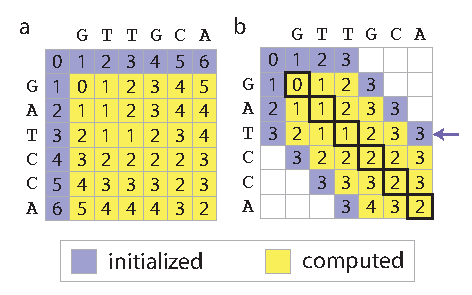
\includegraphics{Fig1.pdf}}
\caption{Needleman-Wunsch (NW) alignment. \textbf{a}
  Alignment of GTTGCA and GATCCA using
the NW alignment matrix. The margins (purple) are initialized and the cells of
the matrix (yellow) are computed from left to right and from top to bottom by a
dynamic programming algorithm. The Levenshtein distance distance between the two
sequences is found in the bottom right cell. \textbf{b}
Lower complexity algorithm to
determine whether GTTGCA and GATCCA are 2-neighbors. The values in purple cells
are set during initialization. The dynamic programming algorithm proceeds as above,
with the difference that it is interrupted if the value of a diagonal cell (bold
borders) is larger than 2. The values in purple cells are not always the same as
their equivalent in a (purple arrow), but the values in the yellow cells are
nevertheless identical. The values of the white cells are never computed, which
contributes to making the algorithm less complex.}\label{fig:01}
\end{figure}

In many instances, the information of interest is whether the sequences are
$d$-neighbors (separated by a distance less than or equal to a threshold $d$).
In that case, the complexity can be reduced to $O(d\cdot \min(m,n))$ as described
below \citep{ukkonen}. Instead of initializing the margins and computing all the
terms, the matrix is initialized as shown on Figure~\ref{fig:01}b and only the
terms around
the diagonal are computed. If the computation of a diagonal term yields a value
greater than $d$, the process is halted (and the distance is known to be greater
than $d$). Otherwise, the distance is the bottom-right term, as in the NW
algorithm.

This method can be used for inexact matching of a sequence against a reference
set indexed as a trie, also called prefix trie \citep{ukkonen}. The terms of the
matrix are updated row-wise as a depth-first search traverses the trie from the
root, as illustrated in Figure~\ref{fig:02}. Every time a node is visited, the row
corresponding to its depth is recomputed. If a diagonal term exceeds the threshold
$d$, the depth-first search backtracks to the parent node because the Levenshtein
distance between the query and all the downstream sequences is greater than $d$,
so there are no hits to discover. When the process halts, every tail node
(corresponding to a sequence of the database) on the path of this search is a
$d$-neighbor of the query. This method is efficient because it eliminates large
areas of the search space, and because the NW alignment of the query with each
prefix of the database is computed only once.

\begin{figure}[!tpb]%figure2
\centerline{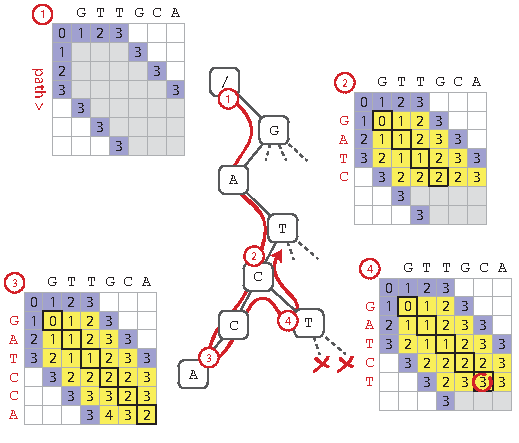
\includegraphics{Fig2.pdf}}
\caption{Trie query with NW alignment. Each sequence of the index is a path in
the trie. The query GTTGCA is written at the top of a NW matrix, which is
initialized as shown on Figure~\ref{fig:01}b. The trie is traversed by a
depth-first search (red path) from the root. At each depth, the node added to
the path is written on the left of the NW matrix and the row is computed.
Checkpoints from 1 to 4 (circled red numbers) show the state of the NW matrix
as the search proceeds. The node labelled 3 is a leaf and thus corresponds to a
2-neighbor of the query. The search path then backtracks to the node labelled 2
and the last rows of the NW are erased. The search path then goes to node labelled
4, in which case the newly computed diagonal cell exceeds the threshold (circled
in red). Even if this node has children, they are not visited (red crosses).}
\label{fig:02}
\end{figure}


\subsection{The poucet search algorithm}
In the case that many sequences are queried only once, this strategy can be
further improved. Notice that if two consecutive queries share a prefix of length
$k$, the sequences of computations up to row $k$ of the NW matrix will be exactly
the same in both queries. Since processing the queries in dictionary order
maximizes prefix sharing, the main idea of the algorithm is to store the
computational intermediates in the nodes of the trie. This way, the search can
start at depth $k$ whenever a query shares a prefix of length $k$ with the previous
one.

However, storing the rows of the NW matrix in the nodes, as suggested by the
approach described in the previous section is not optimal. At depth equal to the
length of the shared prefix, say $k$, the terms on the right of the diagonal were
computed in a previous query using characters that do not belong to the current
query, which means that they would have to be recomputed. Since they also depend
on the terms computed at lower depth, the search cannot restart at depth $k$. This
issue is solved by storing in each node the terms along an angle shape, looking
like a horizontally flipped L character as shown on Figure~\ref{fig:03}. This way, the
computation intermediates stored in a node of depth $k$ depend only on the first
$k$ characters of the query. This means that each query can restart at a depth
equal to the length of the shared prefix with the previous query, thereby
averting the need to recompute the first terms of the NW alignments.

In the fairy tale ``Le Petit Poucet'', the hero seeds white pebbles for his older
brothers to find their way home, which is reminiscent of the way queries pave
 the way for the next in this algorithm. We therefore called this search
algorithm ``poucet''.

\begin{figure}[!tpb]%figure3
\centerline{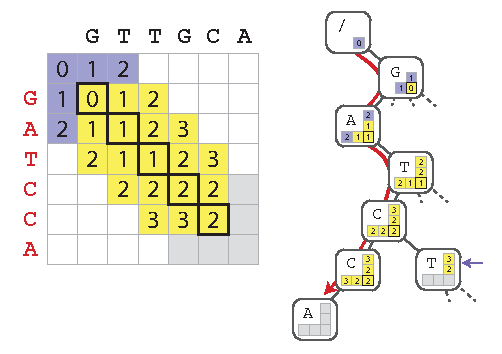
\includegraphics{Fig3.pdf}}
\caption{Poucet search algorithm. The algorithm proceeds with the same principles
as shown on Figure~\ref{fig:02} with the difference that the NW matrix is not
updated row-wise, but along horizontally flipped L shapes. As the depth-first
search proceeds, these values are stored in the nodes of the trie. Only the nodes
at the top contain initialized values; for the other nodes, the values at the
border are implicitly known to be 3. Since the values in the vertical part of
the flipped L are the same for every child of the same node, they are computed
only once (purple arrow). The values in the grey cells will be computed as the
search path (red) visits the node. Storing the intermediates in the nodes allows
the next query to restart at depth $k$ if it shares a common prefix of length
$k$ with the current query.}
\label{fig:03}
\end{figure}


\subsection{Seek and construct}
To reduce the size of the search space, we use a dynamic ``seek and construct''
approach whereby queries are processed meanwhile the trie is built. In other
words, each sequence is matched against the trie before it is inserted. An example
will explain why the trie does not need to contain all the sequences upon query.
Assume that two sequences A and B are $d$-neighbors. A is processed first. Since
B is not yet inserted, A yields not hit. It is then inserted in the trie. At the
time B is processed, A is a hit for the query and the match A-B is discovered.
This approach guarantees that every hit is discovered, while maintaining the
trie as ``thin'' as possible, which reduces search time.
The whole matching process is summarized in the pseudocode shown Figure~\ref{fig:04}

\subsection{Parallelization}
To parallelize the search, queries are separated into contiguous blocks after
sorting, and matching proceeds in two phases. During the first phase, each block
is used as input for the seek and construct process described above. In the second
phase, blocks are queried against the tries built in the first phase. If the
queries are segregated into $N$ blocks, the first phase consists of $N$ seek and
construct jobs, and the second consists of $N(N-1)/2$ query jobs. Since the jobs
show little dependence on each other, the matching algorithm can be efficiently
parallelized provided $N$ is larger than the number of independent threads.

\subsection{Clustering}
Starcode implements a multi-purpose clustering algorithm called ``sphere
clustering'', and a message passing algorithm \citep{mackay} tailored for the
task of clustering random barcodes. In sphere clustering, barcodes are sorted
by frequency and each barcode, starting from the most frequent, can claim its
$d$-neighbors that were not already claimed. This is the method used by
\cite{pmid23953119}.

In message passing clustering, read counts are distributed equally among the
closest neighbors of each barcode if they are at least 5 times more frequent.
The sequences with positive counts at the end of the process are considered
canonical, and their associated count is the estimated cluster size. A barcode
is assigned to a cluster if all its read count are eventually given to the
corresponding canonical barcode. The barcodes for which the read counts are
split between different canonical barcodes are not assigned to any cluster. The
reason for imposing a factor 5 or larger in order to transfer the read counts
is that barcodes with similar frequencies are not likely derived from each other
through sequencing errors. More likely they are either unrelated, or they both
derive from another more abundant barcode.

\subsection{Benchmark options}
The benchmark dataset is described in the Results section. Starcode was run with
options \texttt{-t 20}. CD-HIT version 4.6.1 was run with options
\texttt{-c 0.925 -T 20 -M 0}. USEARCH 32 bit version 7.0.1090 was run with options
\texttt{-threads 20 -cluster\_fast -id 0.925}. The Bowtie2 indexer was run as
\texttt{bowtie2-build --quiet}, and Bowtie2 version 2.1.0 was then run with
options \texttt{-f -a -p 20 --no-hd --very-sensitive}. The BWA indexer was run
as \texttt{bwa index -a is} and then BWA version 0.7.9a was run with options
\texttt{mem -t 20 -a -k1 -B0}. The GEM indexer was first run as
\texttt{gem-indexer -T 20}. GEM version 1.423 (beta) was then run with options
\texttt{-e3 -s -T 20 --granularity 100000}. The sequential algorithm of 
\cite{pmid23953119} was implemented in R and relied on the
\texttt{stringdist}
function of the \texttt{stringdist} package, used with options
\texttt{method='lv', maxDist=2}.

\end{methods}

\section{Results}
\subsection{Benchmark against sequence clustering algorithms}
Sequence clustering is routinely used to curate databases of non redundant
nucleotide or protein sequences. We benchmarked starcode against the two popular
sequence clustering algorithms CD-HIT \citep{pmid23060610} and USEARCH 
\citep{pmid20709691}.

We generated 1 million random 40-mers that were duplicated 47 times. For each
40-mer, we added 3 mutant sequences to the pool by sampling again 3 nucleotides
at random positions. The probability that such a mutant sequence is within a
distance 3 of another 40-mer is of the order of 10-12 and can be neglected.
Each cluster thus consists of 50 sequences, of which 3 have a distance at most
3 from the canonical representant.

Using 20 cores, starcode clustered the shuffled 50 million sequences in 4 minutes
without a single error (the output consisted of 1 million clusters of size 50).
We submitted the unique sequences of the dataset to CD-HIT and USEARCH. The
results are summarized in Figure~\ref{fig:05}. The running times of CD-HIT and USEARCH
were 59 and 64 minutes respectively, and they identified 2,362,352 and 2,739,954
clusters respectively. Both algorithms rely on heuristics, which is why the
number of clusters is off target. These results show that starcode outperforms
other clustering algorithms in speed and accuracy on this particular task.

\begin{figure}[!tpb]%figure5
\centerline{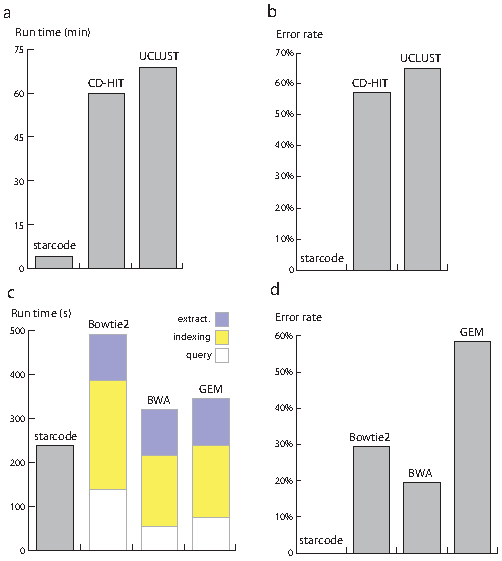
\includegraphics{Fig5.pdf}}
\caption{Benchmark of starcode against sequence clustering algorithms and short
read mappers. \textbf{a} Running time compared to CD-HIT and UCLUST on the
dataset described in the text. \textbf{b} Error rate compared to CD-HIT and UCLUST,
expressed as the percentage of clusters failing to be merged. \textbf{c} Running
time compared to Bowtie2, BWA and GEM on this dataset. The running time is
decomposed in extraction of unique sequences (purple), Burrows-Wheeler indexing
(yellow), and query proper (white). The extraction was performed with the Linux
sort command, so the time is the same in every case. \textbf{d} Error rate compared
to Bowtie2, BWA and GEM, expressed as the proportion of matches with a single hit.
This is an underestimate of the true error rate.}
\label{fig:05}
\end{figure}


\subsection{Benchmark against short read mappers}
A potential strategy to cluster short sequences is to use last generation short
read mappers to match a set of sequences against itself. Once matches are
available, several community detection algorithms can be used to identify the
clusters. We benchmarked starcode against the short read mappers Bowtie2
\citep{pmid22388286}, BWA \citep{pmid19451168} and GEM \citep{pmid23103880}.
Because short read
mappers do not perform clustering, we only evaluated their performance on the
matching problem.

For this test, we used again the dataset described above, in which every
sequence has at least 2 distinct matches at a distance 3. This means that we
can use matches with a single hit (themselves) as a lower bound on the inaccuracy.
We used unique sequences to build an index and queried the index with the same
sequences. Figure~\ref{fig:05} shows the running time of starcode along with the
decomposition of the running time for the three mappers. Note that time to
extract unique sequences is always the same because we used the Linux
\texttt{sort -u} command in every case. It appears that the running time of
starcode is about the same as the time required by BWA (the fastest aligner in
this test) to index and run the query proper. Figure~\ref{fig:05} shows the
lower bound on
the error rate, as estimated by the proportion of single hits. BWA was found to
be the most accurate aligner with a lower bound of 19\% errors. This measure
is an underestimate of the true error rate, but given that starcode makes no
mistake on this dataset, a more accurate measure is not necessary. In conclusion,
starcode runs slightly faster than short read mappers when all steps are taken
into account, and clearly outperforms them in precision on this particular problem.

\subsection{Clustering TRIP barcodes}
In the course of setting up the TRIP technology in our lab \citep{pmid23953119}, we
realized the need to develop efficient algorithms to cluster similar sequences.
Briefly, the principle of TRIP (Thousands of Reporters Integrated in Parallel)
is to tag reporter transcripts with random barcodes and measure the abundance
of barcodes in the RNA as a proxy for gene expression. There is no reference to
match aberrant barcodes against, because the tagging sequences are unknown.
Instead, barcodes are matched against each other and clustered by similarity to
infer canonical sequences.

We tested the efficiency of starcode on the TRIP dataset from
\cite{pmid23953119}. In the experiment labelled mPGKA, we identified
24.1 million barcode-containing reads out of 26.6 million (91\%), consisting
of approximately 223,000 and 220,000 unique barcode sequences for replicates
1 and 2 respectively. Following the authors, we kept only the barcodes with
at least 5 counts and performed clustering as described: ``First we sorted
barcodes according to their counts. Then, for each barcode (starting from the
most frequent one), we identified and removed all its mutant versions, defined
as barcodes within a Hamming distance of 2.'' This method is here on referred
to as the ``sequential algorithm''. When replacing the Hamming distance by the
Levenshtein distance, starcode produced exactly the same output as the sequential
algorithm. The running time of starcode averaged over the replicates was
2.90 seconds, instead of more than 3 minutes 40 seconds, which represents a
75 fold speedup.

The performance of the sequential algorithm relies on the arbitrary exclusion
of reads with less than 5 counts, the main purpose of which is to reduce the
computational burden. When all barcodes were kept, the average running time of
starcode was 10.27 seconds, versus $>$ 6 hours for the sequential algorithm.
Using the Hamming distance as the authors originally suggested decreased the
average running time of the sequential algorithm to 3 hours and 30 minutes (and
the output differed from that of starcode). Note that in all the cases
mentioned above, starcode was run with a single core to compare the algorithms
based on similar computer resources. In conclusion, the barcode clustering
problem can be simplified by various heuristics, but starcode brings down the
running time to nearly instantaneous, and thereby obviates the need for such
arbitrary heuristics.

\subsection{Identifying enriched sequence motifs}
Sequence motifs are thought to play an important role in DNA metabolism. Key
regulators such as transcription factors, nucleosomes and non coding RNAs have
sequence preferences targeting them to the sites where they act. Identifying
those sequences is a way to pinpoint the regulators and the mechanisms they
are involved in. However, the sequence motifs are not strictly identical
between sites, which is why they are better identified by inexact matching.
This problem becomes computationally difficult for long motifs (above 12-13
nucleotides) because of the combinatorial explosion. But as motifs become
longer, the problem of identifying abundant inexact matches becomes similar
to barcode clustering.

We set up a test based on the meningitis-causing agent
\textit{Neisseria meningitidis}. The genome of this bacterium is interspersed
with a frequent 12 bp sequence known as DNA uptake sequence \citep{pmid10673000}. We
extracted the 12-mers from both orientations of �the 2.19 Mb genome, yielding
4.39 million 12-mers, consisting of 2.77 million unique sequences. Using
starcode to cluster the 12-mers within a Levenshtein distance of 2 took less
than 3 minutes with 20 cores. We identified the known DNA uptake sequence of
Neisseria meningitidis (ATGCCGTCTGAA) as the most abundant 12-mer, comprising
1,466 exact matches and 4,625 inexact matches. This shows that starcode can
be used to identify biologically relevant motifs in bacterial genomes.

To test starcode on the scale of a metazoan genome, we used a Drosophila
dataset from \cite{pmid20888037}. That study describes two
signatures of chromatin proteins called Red and Yellow, that both correspond
to transcribed regions of the genome. The distinction is based on epigenomic
features only, which prompted us to identify sequence features that could
discriminate Red versus Yellow regions. To this end, we used starcode to
cluster 18-mers from both regions.

The total coverage of Red and Yellow chromatin in the Drosophila genome is
10.7 and 21.3 Mb respectively, corresponding to 21.5 million and 42.5 million
18-mers respectively. We used starcode to identify clusters of 18-mers within
a Levenshtein distance of 3 (the running time was approximately 35 minutes for
Red 18-mers and 70 minutes for Yellow 18-mers using 20 cores). The frequencies
of the most abundant 18-mers showed that Red chromatin has a lower sequence
complexity than Yellow chromatin (not shown). The most discriminating 18-mer
was (GA)$_9$, which showed a 4.8 fold enrichment in Red versus Yellow chromatin.
We counted 832 exact matches and 6,749 inexact matches (over 3,880 distinct
18-mers) in Red chromatin, showing that a larger portion of the signal comes
from inexact matches. Taken together, these results show that starcode can be
used to cluster short k-mers from metazoan-scale datasets.


\section{Discussion and conclusion}
Through the parallel poucet search algorithm, starcode implements an exact
sequence clustering algorithm that is even faster than widely used heuristics.
By design, starcode is tailored to process high throughput sequencing data on
multi-core platforms. Our benchmark shows that starcode is superior in speed
and accuracy to other methods on the problem of clustering short random
sequences. Part of the reason is that this task is stretching the tested
software far from their initial design. Sequence clustering algorithms are
meant to to cluster long biological sequences, while short read mappers are
meant to map reads on potentially large genomes. In this respect, starcode
fills a need arising from the development of barcoding technologies.

The speed of starcode also makes it proficient at more general clustering
problems, such as identifying enriched k-mers in genomes and in experimental
data. Here we have given two examples of such applications. In the first, we
recover a known enriched 12-mer in the genome of \textit{Neisseria meningitidis}.
In the second, we identify a sequence feature that discriminates genomic
regions found in two different chromatin types in Drosophila. GA repeats are
known to be bound in vivo by the protein GAF \citep{pmid12601174}, which suggests
that this transcription factor is instrumental in setting the distinction
between Red and Yellow chromatin.

The current version of starcode has been mildly optimized for memory
consumption. The memory footprint depends on the number of sequences to
cluster (because the sequences of the input set are loaded in memory as a
group of tries) and on the mean number of matches per sequence. Every match
has to be stored until the clustering phase, which can represent a heavy
load. As counterintuitive as it may seem, long queries will usually impose
a lower memory footprint because the matches between sequences are less
frequent.

The speed of starcode could benefit other applications, such as searching
shared subsequences in genome assembly. However, starcode supports only global
and not local alignment. A work around is to compare k-mers as we have done
in the examples above, but this approach is expected to be memory demanding.
Extending the starcode algorithm to support clustering of protein sequences
is straightforward but the speed is not expected to meet the level of the
algorithm shown here. On the one hand, there are more letters in the protein
alphabet, so the shared prefix between consecutive queries is expected to be
shorter on average, which defeats the poucet search. On the other hand, if
a threshold distance of the order of 1 per 10 nucleotides is sufficient to
identify similar DNA sequences, a distance of 1 per 10 residues is
unrealistically low for protein sequences, and this parameter critically
determines the speed of starcode. More generally, storing computational
intermediates for shared prefixes could find some applications in other
algorithms such as short read mappers. The idea of the poucet search seems
simple in retrospect, but it is a powerful way to tap into the data
structuration provided by string sorting.







%%%%%%%%%%%%%%%%%%%%%%%%%%%%%%%%%%%%%%%%%%%%%%%%%%%%%%%%%%%%%%%%%%%%%%%%%%%%%%%%%%%%%
%
%     please remove the " % " symbol from \centerline{\includegraphics{fig01.eps}}
%     as it may ignore the figures.
%
%%%%%%%%%%%%%%%%%%%%%%%%%%%%%%%%%%%%%%%%%%%%%%%%%%%%%%%%%%%%%%%%%%%%%%%%%%%%%%%%%%%%%%


\section*{Acknowledgement}
We would like to thank...

\paragraph{Funding\textcolon}
The research leading to these results has received funding from the
Government of Catalonia (Dept. of Economy and Knowledge) and the Spanish
Ministry of Economy and Competitiveness (Centro de Excelencia Severo Ochoa
2013-2017' (SEV-2012-0208). P.C. fellowship is partly financed by the
Spanish Ministry of Economy and Competitiveness (State Training Subprogram:
predoctoral fellowships for the training of PhD students (FPI) 2013).

\bibliographystyle{natbib}
%\bibliographystyle{achemnat}
%\bibliographystyle{plainnat}
%\bibliographystyle{abbrv}
%\bibliographystyle{bioinformatics}
%
%\bibliographystyle{plain}
%
\bibliography{document}


%\begin{thebibliography}{}
%\end{thebibliography}
\end{document}
